\documentclass[12pt]{article}

\usepackage{amsmath}
\usepackage[super]{nth}
\usepackage[utf8]{inputenc}
\usepackage[T1]{fontenc}
\usepackage{textcomp}
\usepackage{gensymb}
\usepackage{graphicx}
\usepackage{hyperref}
\usepackage{caption}
\usepackage{float}

\pagenumbering{arabic}

\begin{document}

\title{Graphical Analysis - Literature Study}
\date{December 06, 2016}
\author{Rafael De Smet}

\maketitle
\tableofcontents
\newpage
\section{Introduction}

In this paper I will be discussing several graphical analysis algorithms. These algorithms will return data which are used to base the music generation on. Not all algorithms are used in the code, but are discussed for the sake of completeness. Besides the image processing algorithms I will be discussing text recognition as well.

\section{Image Processing Algorithms}

\subsection{Edge Detection}

The concept of edge detection is pretty straightforward. The algorithms try to detect all the edges in an image. Edges are the contours of objects and shapes in the image.
Edge detection algorithms all use what are called convolution kernels. A kernel in image processing is a small matrix used to apply effects to an image, such as blurring and outlining. Here we will see kernels used for edge detection only. Listed below are six of the best and most used algorithms.

\begin{itemize}
        \item Sobel 
        \item Frei-Chen
        \item Prewitt
        \item Roberts Cross
        \item LoG
        \item Scharr
\end{itemize}

\subsubsection{Convolution kernel}

Convolution is the technique of multiplying together two arrays of different size but of the same dimension. An array of dimension two simply is a matrix. When working with images the pixels are represented as a (2D) matrix and the kernel is also a 2D matrix.
The kernel is a small matrix that we will multiply with the image matrix to perform the convolution. This kernel matrix is different for each edge detection algorithm. We will see examples of different matrices later in this paper. 
\newline

The idea of these algorithms is to create a new image that shows the edges of the original image. Each pixel of the original image is added to its local neighbours, weighted by the kernel. This produces a new image. The result of the matrix multiplication results in new pixel values that denote the edges of the image. 
Mathematically we can write the convolution as follows, with $O$ the output image, $I$ the input image and $K$ the kernel. $I(i,j)$ means the pixel on the $i^{th}$ row and the $j^{th}$ column.

\begin{equation}
O(i, j) =  \sum\limits_{k=1}^m\sum\limits_{l=1}^n I(i + k - 1, j + l - 1)K(k,l)
\end{equation}
\newline

An example will clarify the previous.

\begin{figure}[h]
\centering
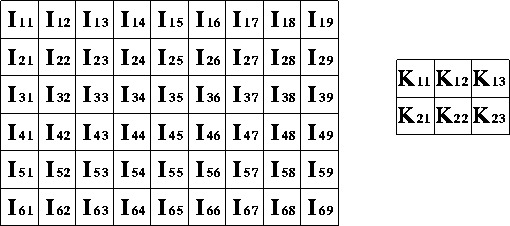
\includegraphics[scale = 0.5]{img/convolution}
\caption{A pixel matrix and a kernel matrix}
\label{kernel}
\end{figure}

Using the kernel matrix we will compute every new pixel of the output image, by sliding the kernel matrix over the original pixels. Each kernel position corresponds to a single output pixel, the value of which is calculated by equation (1).
\newline

In our example, the value of the bottom right pixel in the output image will be found as follows [2]:

\begin{equation}
O_{57} = I_{57}K_{11} + I_{58}K_{12} + I_{59}K_{13} + I_{67}K_{21} + I_{68}K_{22} + I_{69}K_{23}
\end{equation}
\newpage

In figure \ref{picasso} you can see a painting by Picasso. We will use this image to see how well the different edge detection algorithms work.

\begin{figure}[h]
\centering
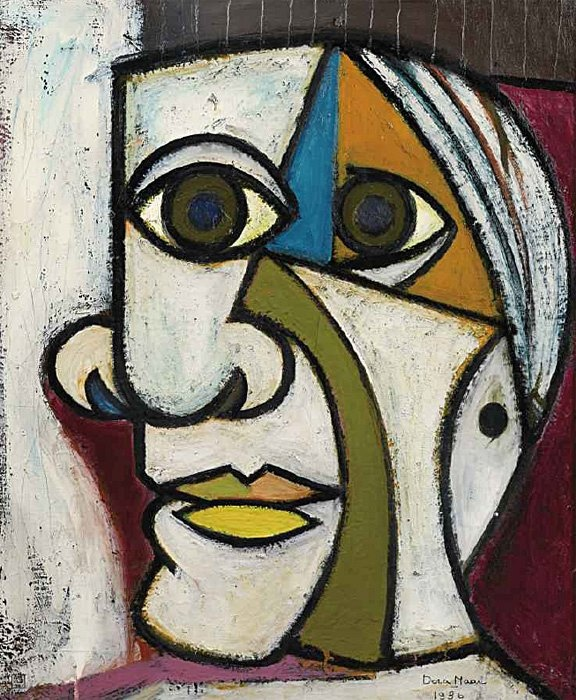
\includegraphics[scale = 0.39]{img/picasso}
\caption{Picasso}
\label{picasso}
\end{figure}

\subsubsection{Sobel}

 The Sobel algorithm performs a 2D spatial gradient measurement and defines regions of 'high spatial frequency' or edges. It uses two 3x3 kernels, one for the horizontal edges and one for the vertical edges. These two kernels are applied consecutively and the results are combined to define all the edges. In figure \ref{sobel} you can see the result of the Sobel filter.
 \newline

 The horizontal kernel: 
 $\begin{vmatrix}
        -1 & 0 & +1\\
        -2 & 0 & +2\\
        -1 & 0 & +1\\
\end{vmatrix}$
and the vertical kernel:
$\begin{vmatrix}
        +1 & +2 & +1\\
        0 & 0 & 0\\
        -1 & -2 & -1\\
\end{vmatrix}$

\begin{figure}[h]
\centering
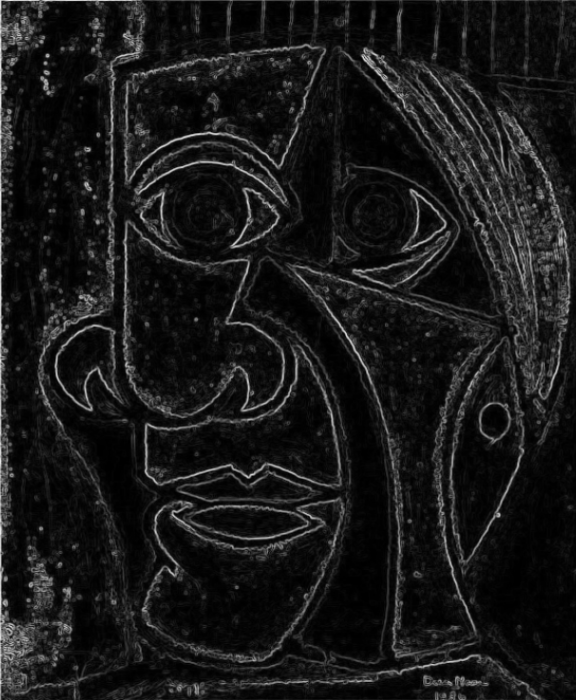
\includegraphics[scale = 0.39]{img/picassoSobel}
\caption{Sobel filter applied to figure \ref{picasso}}
\label{sobel}
\end{figure}
\newpage

\subsubsection{Frei-Chen}
 The Frei-Chen algorithm also uses 3x3 kernels, but this time there are nine different convolution kernels. The four first matrices, G1, G2, G3, G4, are used for edges, the next four are used for lines and $G_9$ is used to compute averages. $G_9$ attenuates the impact of the computations from the other matrices. Figure \ref{freichen} shows the result of the Frei-Chen filter.
\newline
\newline
 $G_1$ = $\frac{1}{2\sqrt2}$ $\begin{vmatrix}
        1 & \sqrt2 & 1\\
        0 & 0 & 0\\
        -1 & -\sqrt2 & -1\\
\end{vmatrix}$\hspace{5mm}
$G_2$ = $\frac{1}{2\sqrt2}$$\begin{vmatrix}
        1 & 0 & -1\\
        \sqrt2 & 0 & -\sqrt2\\
        1 & 0 & -1\\
\end{vmatrix}$\hspace{5mm}
$G_3$ = $\frac{1}{2\sqrt2}$$\begin{vmatrix}
        0 & -1 & \sqrt2\\
        1 & 0 & -1\\
        -\sqrt2 & 1 & 0\\
\end{vmatrix}$\hspace{5mm}
\newline
$G_4$ = $\frac{1}{2\sqrt2}$$\begin{vmatrix}
        \sqrt2 & -1 & 0\\
        -1 & 0 & 1\\
        0 & 1 & -\sqrt2\\
\end{vmatrix}$\hspace{5mm}
$G_5$ = $\frac{1}{2}$$\begin{vmatrix}
        0 & 1 & 0\\
        -1 & 0 & -1\\
        0 & 1 & 0\\
\end{vmatrix}$\hspace{10mm}
$G_6$ = $\frac{1}{2}$$\begin{vmatrix}
        -1 & 0 & 1\\
        0 & 0 & 0\\
        1 & 0 & -1\\
\end{vmatrix}$\hspace{5mm}
\newline
$G_7$ = $\frac{1}{6}$$\begin{vmatrix}
        1 & -2 & 1\\
        -2 & 4 & -2\\
        1 & -2 & 1\\
\end{vmatrix}$\hspace{13mm}
$G_8$ = $\frac{1}{6}$$\begin{vmatrix}
        -2 & 1 & -2\\
        1 & 4 & 1\\
        -2 & 1 & -2\\
\end{vmatrix}$\hspace{11mm}
$G_9$ = $\frac{1}{3}$$\begin{vmatrix}
        1 & 1 & 1\\
        1 & 1 & 1\\
        1 & 1 & 1\\
\end{vmatrix}$\hspace{5mm}

\begin{figure}[h]
\centering
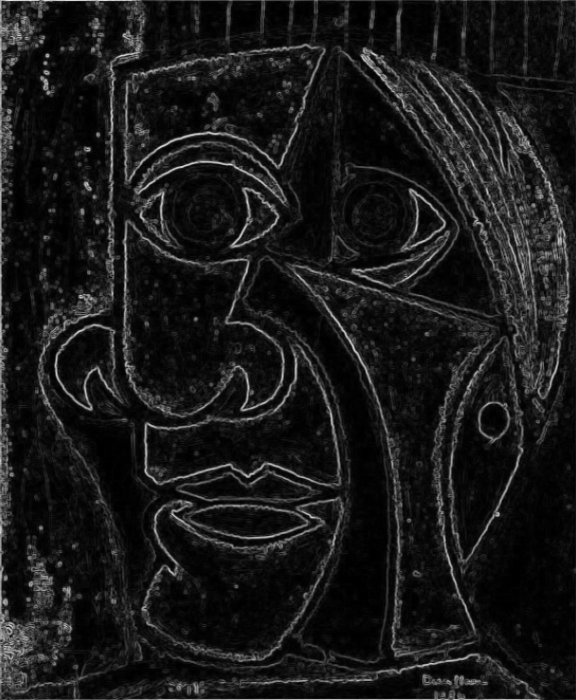
\includegraphics[scale = 0.39]{img/picassoFreiChen}
\caption{Frei-Chen filter applied to figure \ref{picasso}}
\label{freichen}
\end{figure}

\subsubsection{Prewitt}
This algorithm is very similar to the Sobel algorithm. Again, two kernels are used, one for the horizontal and one for the vertical edges. In this case the kernels are basic convolution filters of the following form. 
\newline

Horizontal filter = $\begin{vmatrix}
        1 & 1 & 1\\
        0 & 0 & 0\\
        -1 & -1 & -1\\
\end{vmatrix}$\hspace{11mm}
Vertical filter = $\begin{vmatrix}
        -1 & 0 & 1\\
        -1 & 0 & 1\\
        -1 & 0 & 1\\
\end{vmatrix}$
\newline

\begin{figure}[h]
\centering
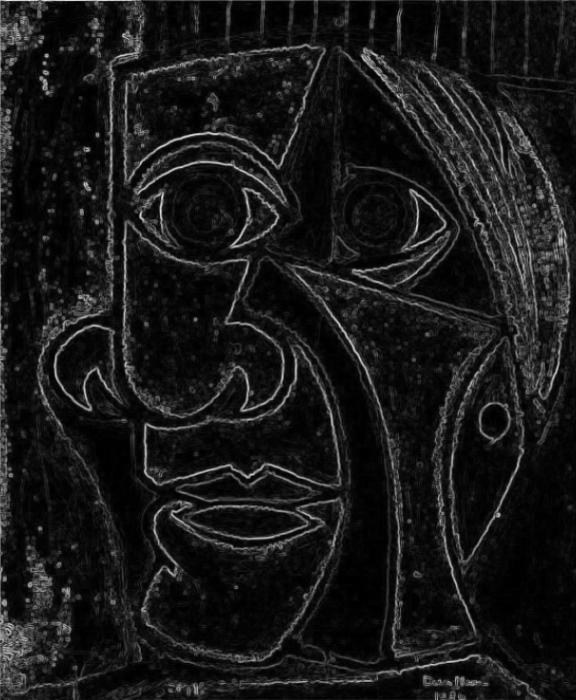
\includegraphics[scale = 0.39]{img/picassoPrewitt}
\caption{Prewitt filter applied to figure \ref{picasso}}
\label{prewitt}
\end{figure}
\newpage

\subsubsection{Roberts Cross}
This algorithm uses even simpler kernels than Prewitt does. This time we use two 2x2 kernels. These kernels correspond to the edges running at 45° to the pixel grid, one for each of the two perpendicular orientations. Figure \ref{robertscross} shows the result of the Roberts Cross filter.
\newline

Horizontal filter = $\begin{vmatrix}
        1 & 0 \\
        0 & -1 \\
\end{vmatrix}$\hspace{11mm}
Vertical filter = $\begin{vmatrix}
        0 & 1\\
        -1 & 0\\
\end{vmatrix}$

\begin{figure}[h]
\centering
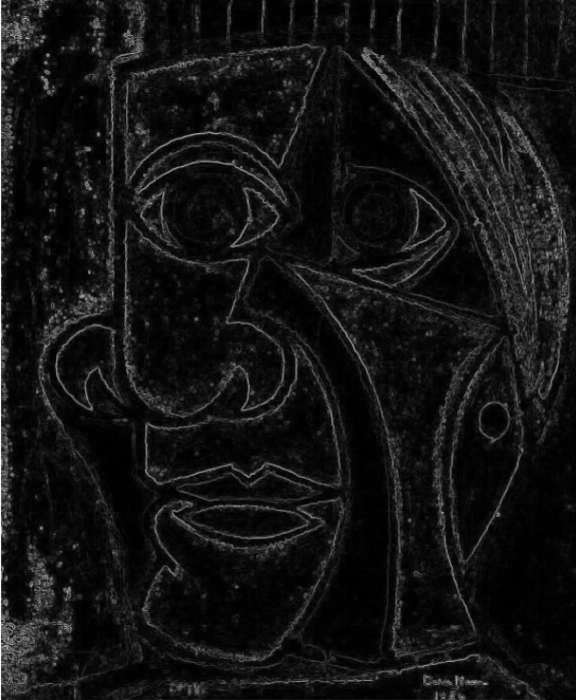
\includegraphics[scale = 0.39]{img/picassoRobertsCross}
\caption{Roberts Cross filter applied to figure \ref{picasso}}
\label{robertscross}
\end{figure}

\subsubsection{LoG}
This algorithm first applies Gaussian filtering\footnote{The Gaussian filter is used to blur images and remove noise and detail.} to the image and then the Laplacian method for edge detection\footnote{The Laplacian method highlights regions in the image of rapid intensity change, so it is useful for edge detection.}, hence the name "Laplacian of Gaussian" (LoG).
The edge points of an image are detected by finding the zero crossings of the \nth{2} derivative of the image intensity. Because the \nth{2} derivative is very sensitive to noise, which could give us bad results, the Gaussian filter is used to clear the noise from the image. In figure \ref{log}, you can find the result of this filter.
\newline

The R library OpenImageR\footnote{https://cran.r-project.org/web/packages/OpenImageR/OpenImageR.pdf} uses the following LoG mask.
\newline

LoG mask = $\begin{vmatrix}
        1 & 1 & 1\\
        1 & -8 & 1\\
        1 & 1 & 1\\
\end{vmatrix}$

\begin{figure}[h]
\centering
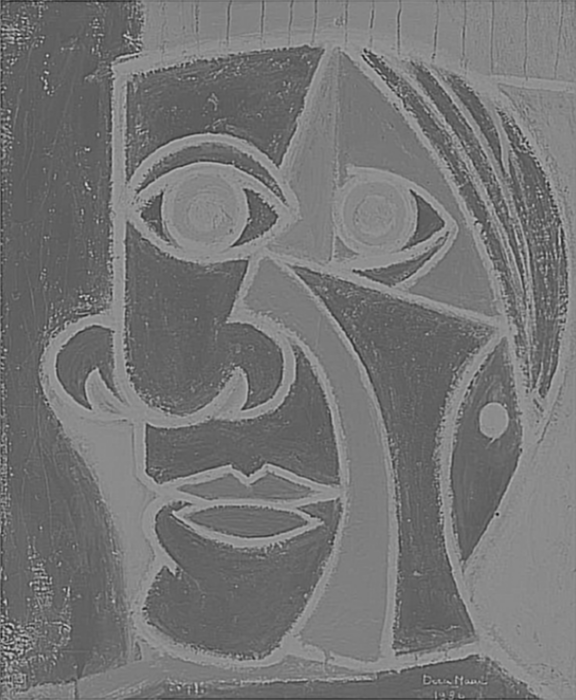
\includegraphics[scale = 0.39]{img/picassoLoG}
\caption{LoG filter applied to figure \ref{picasso}}
\label{log}
\end{figure}

\subsubsection{Scharr}
The last algorithm is again an extension of the Sobel algorithm. This operator improves rotational invariance, which means that if the image is rotated, the operator should define the same edges. Sobel can have difficulties with this aspect. There are many Scharr kernels, some even 5x5, but the following are most frequently used. Figure \ref{scharr} shows the results.
\newline

Horizontal filter = $\begin{vmatrix}
        3 & 10 & 3\\
        0 & 0 & 0\\
        -3 & -10 & -3\\
\end{vmatrix}$\hspace{11mm}
Vertical filter = $\begin{vmatrix}
        3 & 0 & -3\\
        10 & 0 & -10\\
        3 & 0 & -3\\
\end{vmatrix}$\hspace{5mm}

\begin{figure}[h]
\centering
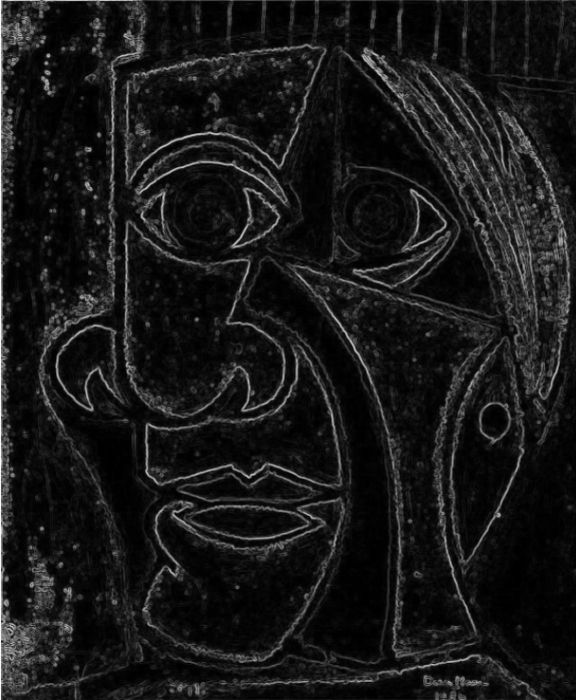
\includegraphics[scale = 0.39]{img/picassoScharr}
\caption{Scharr filter applied to figure \ref{picasso}}
\label{scharr}
\end{figure}
\newpage

\subsection{Noise Removal}

Every edge detection algorithm was based on a specific filter. Using this same idea of applying filters to images we can detect and remove typical noise, such as additive 'salt and pepper' and Gaussian noise. Analogous to the previous section, I will discuss several noise removal algorithms and the filters used. The first image of figure \ref{noise_original} is the image I will be using to discuss the results of the algorithms [14].
\newline

In this section I will be discussing the effects of the filters on two kinds of noise. The first is the 'salt and pepper' noise, of which you can see an example in the second image of figure \ref{noise_original}. Secondly, we have the Gaussian noise, the third image in figure \ref{noise_original}

\begin{figure}[h]
\hspace*{-0.8cm}
\centering
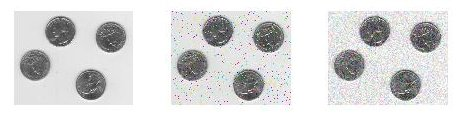
\includegraphics[scale = 1]{img/noise_orig}
\caption{Original image, 'salt and pepper' noise, Gaussian noise}
\label{noise_original}
\end{figure}

\subsubsection{Mean filtering}

This is the simplest linear filter of them all and operates by giving weight $w_K$ to all the pixels in the neighbourhood of a certain pixel. Let's say we have a $N\times M$ neighbourhood, then we define the weight as follows: $w_K = \frac{1}{NM}$. The filter used in this technique is a $3\times3$ filter. Below you can see the filter I used to generate the results.
\newline

Mean filter:
$\begin{bmatrix}
	0.1111 & 0.1111 & 0.1111 \\
	0.1111 & 0.1111 & 0.1111 \\
	0.1111 & 0.1111 & 0.1111 \\
\end{bmatrix}$
\newline

In figure \ref{noise_mean} you can see the results of this filter. We can see that the filter is reasonably effective at removing the Gaussian noise (third image), but at the expense of losing detail in the edges of the image. The filter is not effective for the removal of the 'salt and pepper' noise. This is caused by a large deviation of the noise values from the typical values in the neighbourhood. This means that the average value is significantly influenced. This deviation is still very visible in the result.
\newline

The main disadvantages of mean filtering are (a) it is not robust to large noise deviations (also called outliers) and (b) the edges in the images will be blurred. This suggests we should look at a more robust (to statistical outliers) filter.

\begin{figure}[h]
\hspace*{-2cm}
\centering
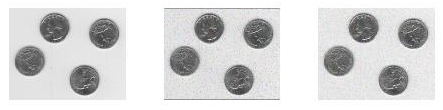
\includegraphics[scale = 1.2]{img/noise_mean}
\caption{Original image with mean filter, 'salt and pepper' noise with mean filter, Gaussian noise with mean filter}
\label{noise_mean}
\end{figure}

\subsubsection{Median filtering}

Where the mean filtering used the mean of a $N \times M$ neighbourhood as the weight, this filtering uses the statistical median of the neighbourhood. This filter is better than the mean filter because it preserves edges better whilst eliminating noise. The advantage of using the median is the fact that it is more robust to statistical outliers and does not create new unrealistic pixel values.
\newline

The disadvantage of this method is the high computational requirement. To calculate the median of values, it requires an ordering of those values, in this case the pixel values.
\newline

In figure \ref{noise_median} you can see the results of this filter. It is clear that the median filter is very effective at removing the 'salt and pepper' noise. The removal of the Gaussian noise still is at the expense of a sloght degradation in image quality. 

\begin{figure}[h]
\hspace*{-1.7cm}
\centering
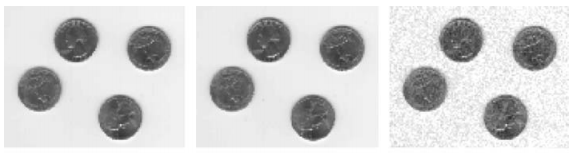
\includegraphics[scale = 0.9]{img/noise_median}
\caption{Original image with median filter, 'salt and pepper' noise with median filter, Gaussian noise with median filter}
\label{noise_median}
\end{figure}

\subsubsection{Rank filtering}

The median filter is nothing more than a special case of this generalized order (rank) filter [14]. A general order linear filter follows four common steps.

\begin{itemize}
\item Define neighbourhood of the target pixel ($N\times N$).
\item Rank them in ascending order.
\item Choose the order of the filter.
\item Set the filtered value to be equal to the value of the chosen rank pixel.
\end{itemize}

A common practice is to choose the minimum and maximum values of the pixels in the defined neighbourhood. Unsurprisingly, these filters are called minimum and maximum filters. In figure \ref{noise_rank} you can see the results of this filter. The effect of this filter on the 'salt and pepper' noise is not so good. Because the filters selects the maximum and minimun filters, the high values in the image are amplified. The effects on the Gaussian noise are better, the noise is largely removed, but at the cost of image detail.

\begin{figure}[h]
\hspace*{-1.2cm}
\centering
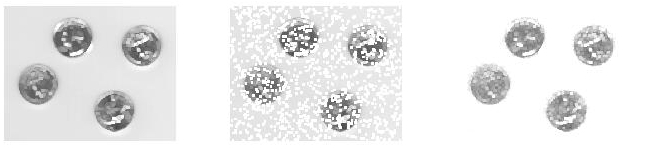
\includegraphics[scale = 0.8]{img/noise_rank}
\caption{Original image with rank filter, 'salt and pepper' noise with rank filter, Gaussian noise with rank filter}
\label{noise_rank}
\end{figure}

\subsubsection{Gaussian filtering}

This technique differs from the other three I discussed. The filter used is a discrete kernel derived from a radially symmetric form of the continous 2D Gaussian function defined as follows [14]:

\begin{equation}
f(x,y) = \frac{1}{2\pi \sigma ^2} exp(-\frac{x^2 + y^2}{2\sigma^2})
\end{equation}
\newline

Applying the Gaussian filter has the effect of smoothing the image. This smoothing has two interesting characteristics. First, the degree of smoothing is controlled by the choice of the standard deviation $\sigma$. Secondly, the Fourier transform of the Gaussian function is a Gaussian function itself. This means that it is very convenient for the frequency-domain analysis of filters, but that discussion is out of the scope of this paper.
\newline

In figure \ref{noise_gaussian} you can see the results of this filter. In all cases, the smoothing effect causes the edges to fade a little, but it also removes the noise to a certain degree. For this result I used a Gaussian filter with $\sigma = 2$. This filter gives us the best of all the previous filters, with the median filter a close second choice.

\begin{figure}[h]
\hspace*{-1.2cm}
\centering
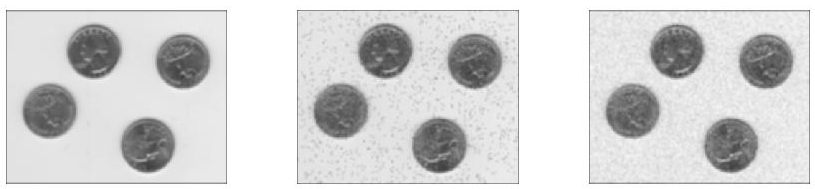
\includegraphics[scale = 0.6]{img/noise_gaussian}
\caption{Original image with Gaussian filter ($\sigma = 2$), 'salt and pepper' noise with Gaussian filter, Gaussian noise with Gaussian filter}
\label{noise_gaussian}
\end{figure}
\newpage

\subsection{Color Analysis}
Only edge detection algorithms are not sufficient to get enough data from the image to form a musical interpretation. We will need some form of color analysis as well. This section describes some algorithms and methods to obtain information about the colors of the image.

\subsubsection{RGB - HSV - CMYK}
To represent color on the computer the RGB representation is the most commonly used. Each pixel is described using three values, the amount of red (R), green (G) and blue (B). Using these values we can count how many pixels in the image are dominantly red, green or blue. When we're going to translate the image data into musical patterns, we can match each color to another kind of music (happy, sad, etc...)
\newline

HSV, sometimes called HSB, is another representation of a pixel. This time we use the hue (color, denoted by H), the saturation (S) and the brightness or value (B or V) to describe the pixel. Where the RGB model consists of three values indicating the amounts of a certain color each pixel has, the HSV model consists of three independent components to form a color. 
\newline

\paragraph{Hue} First we have the hue, which is the color. The color is represented using a circle with all the colors on it. The value of this component is the degrees of the angle we have to make on the circle to get this color.  

\paragraph{Saturation} The saturation indicates the fullness of the color. This value is expressed in a percentage, with 0\% a gray, flat color and 100\%  a full, rich color.

\paragraph {Value of Brightness} The value or brightness indicates the amount of light of the color and is also expressed in a percentage, 0\% is black and 100\% is white.

\begin{figure}[h]
\centering
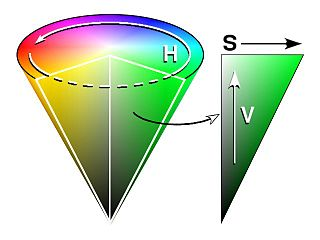
\includegraphics[scale = 0.45]{img/hsv}
\caption{The HSV color representation}
\label{hsv}
\end{figure}

CMYK is another representation of color, based on the mixing of four colors, cyan (C), magenta (M), yellow (Y) and key (K, black). This model is used frequently with printing, but not very interesting for this paper.

\subsubsection{Black And White Balance}
During the image analysis we will convert the image to a gray scale image, so we can determine the amount of white and black in it. Using the RGB model, this is an easy process. Black in the RGB model is (0,0,0) and white is (255,255,255). So we can simply count the amount of pixels that are very close to those two values and we know the amount of black and white pixels in the image.
Analogous to this we can count every gray pixel in the image, by finding every pixel where the RGB values are exactly the same.

\subsubsection{Color Quantization (Image Segmentation)}

Sometimes it can be easier to work with images that are partitioned in simpler regions. This technique is called color quantification or image segmentation. There are many different ways to implement this technique. One such approach is using the k-means cluster algorithm. This algorithm attempts to partition a data set into $k$ clusters. The data set contains the RGB values of each pixel.
The disadvantage of this algorithm is that we don't know what the right value for $k$ is. So we have to perform this algorithm a couple of times, each time with a different k $k$ to see which value gives us a good result.
\newline

A second technique is the X-means algorithm which is an improvement of the k-means algorithm. The X-means algorithm can determine the number of clusters by itself, using the Bayesian information criterion (BIC). BIC is a selection criterion for clustermodels. Based on the total number of clusters found by X-means, we can generate parts of the piece of music.
\newline

To illustrate this technique, you can find in figure \ref{mandrill} an image of a mandrill. Using the k-means algorithm we can break this image in four color regions [13]. This means $k = 4$. The result of this segmentation can be found in figure \ref{mandrill_segmented}. It is clear to see that we have found 4 dominant colors: red, lightblue, gray and darkgray (almost black). We can get a better understanding of color quantization by visualizing our image in the color space. In figure \ref{colorspacemandrill} you can see the four dominant colors resulting from the algorithm.  

\begin{figure}[H]
\centering
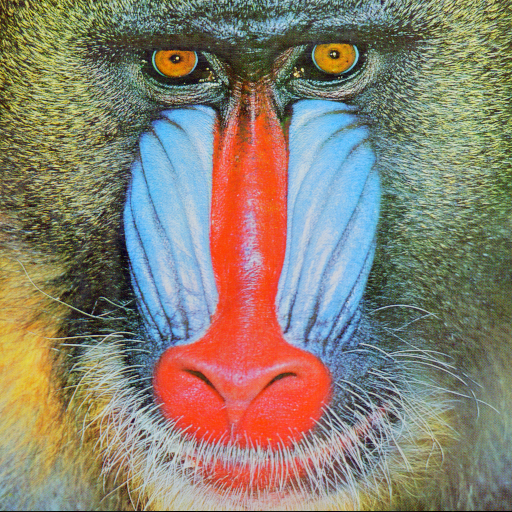
\includegraphics[scale = 0.39]{img/mandrill}
\caption{Mandrill image}
\label{mandrill}
\end{figure}

\begin{figure}[H]
\centering
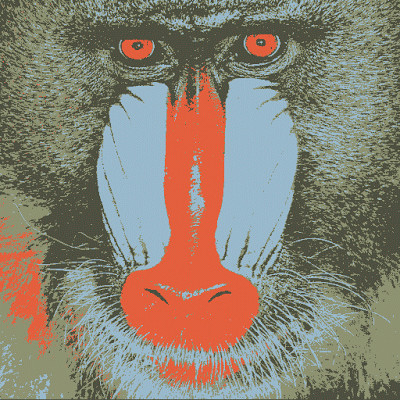
\includegraphics[scale = 0.5]{img/mandrill_segmented}
\caption{Mandrill image segmented}
\label{mandrill_segmented}
\end{figure}

\begin{figure}[H]
\centering
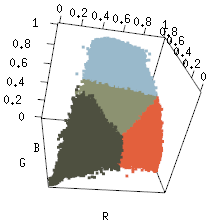
\includegraphics[scale = 0.9]{img/colormandrill-11}
\caption{Segmented mandrill image in color space}
\label{colorspacemandrill}
\end{figure}

\subsection{Image Hashing}
It is also possible to get the hash value of an image. The hash is a hexadecimal number and is another representation of the image. This is used to compare images. 

\subsubsection{Average Hashing}
The first hash method is the average hash of the image. This algorithm contains five steps.

\begin{enumerate}
        \item Convert the image to grayscale. 
        \item Reduce the size of the image, to reduce the number of computations.
        \item Average the resulting colors. For an 8x8 image, 64 will be averaged.
        \item Compute the bits of the hash value by comparing if each color value is above or below the mean.
        \item Construct the hash.
\end{enumerate}

\subsubsection{Difference Hash}
We can also compute the dHash of an image. It is similar to the average hash, but now the difference between adjacent pixels is also considered in the computation.

\subsubsection{Perceptive Hash}
This method uses the discrete cosine transform (DCT) and compares the pixels based on the frequencies, given by the DCT, instead of the color values.
DCT is a similar technique as Fourier analysis, it expresses a finite sequence of points, in this case the pixels, in terms of a sum of cosine functions.

\subsubsection{Use Of The Hash}
One application of these methods is the recognition of images. Search engines like Google use this technique to search similar images to any image you provide to the search engine. I could use this as a way to store information about the image my application has already scanned and generated music for.
\newline

In figure \ref{hashtable} you can see the results of applying the three types of hash to three images of a tree. These images are figures \ref{tree1}, \ref{tree2} and \ref{tree3}. It is clear that the average hash produced similar results for every tree, while there is more difference in the results of the difference hash and the perceptive hash.

\begin{figure}[H]
\centering
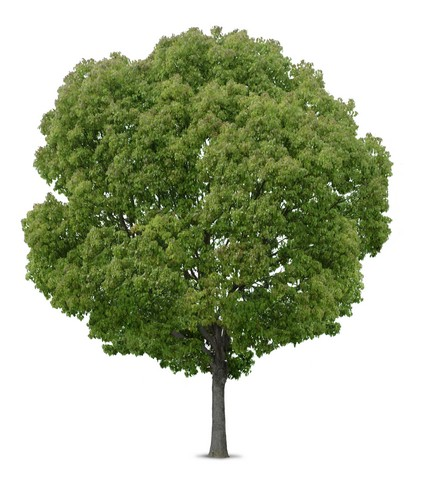
\includegraphics[scale = 1.5]{img/boom1}
\caption{Tree 1}
\label{tree1}
\end{figure}

\begin{figure}[H]
\centering
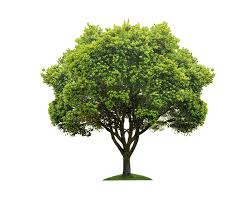
\includegraphics[]{img/boom2}
\caption{Tree 2}
\label{tree2}
\end{figure}

\begin{figure}[H]
\centering
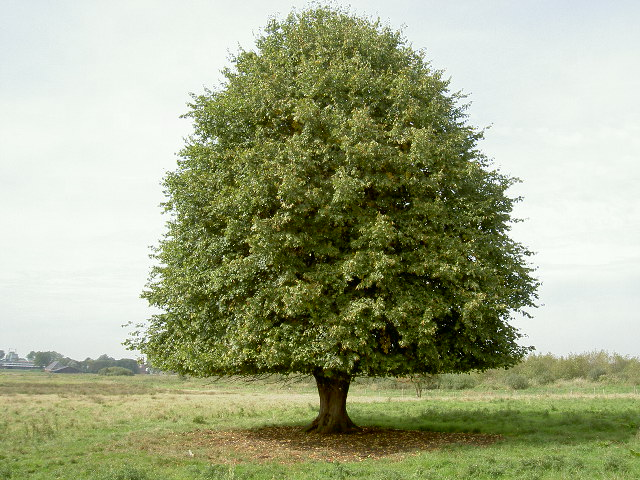
\includegraphics[scale = 0.5]{img/boom3}
\caption{Tree 3}
\label{tree3}
\end{figure}

\begin{figure}
\centering
\begin{tabular}{| c | c | c | c |}
\hline
& \textbf{Average Hash} & \textbf{Difference Hash} & \textbf{Perceptive Hash} \\
\hline
Tree 1 & ffcf8303030187ff & 00007c00b852ec7c & 7f9c2185534b98f1 \\ 
\hline
Tree 2 & ffff8f070707dfdf & 000000e804f8f800 &  4796a9695a6929d6 \\
\hline
Tree 3 & ffdf8f8787078708 & d6878788e300f8f8 & 87a569535b9899c9 \\
\hline
\end{tabular}
\caption{Table of hash results}
\label{hashtable}
\end{figure}

\subsection{Entropy}

Still another method we can use to get information from an image is to calculate the entropy.
The entropy is a measure of the amount of disorder in the image.
\newline

When talking about images, we consider the following. If all the pixels of the image have the same level of a specific parameter, the entropy is zero. This means there is not a lot of information (almost none) to be gained from the image. An image of a blue sky has a very low entropy cause we only see blue. 

When all the pixels in the image are different, the entropy of the image is maximum and there is a lot of information to get from the image. As the entropy describes how much (dis)order there is, we will use this to determine how much (dis)order there is in the generated music.
\newline

To get the right information about the pixels, we use a histogram that shows the count of the distinct pixel values. The entropy of an image $H$ is defined as:
\begin{equation}
H = - \sum_{k=0}^{M-1} p_k log_2 (p_k)
\end{equation}

where M is the number of unique pixel values and $p_k$ is the count of each pixel level, how many times this pixel level occures in the image.
\newline

In the ArtToMusic application we will investigate whether it is useful to use the entropy of the original image in the music generation process. We can as well calculate the entropy of the result of a specific analysis and we expect that this approach will be more beneficial.
\newline

To illustrate the concept of entropy, I have provided two examples. In figure \ref{entropy_picasso} you can see the same painting as I used in the discussion of the edge detection algorithms. The left part of this image shows the original painting. It has quite a lot of information, there is a face with several distinguishable areas, lot of different colours and many edge. The middle part of the image shows the grayscale version of the painting, the algorithm uses this image to calculate the entropy [12]. The right part of the image shows the entropy for every pixel, based on the 10x10 neighbouring pixels. Red indicates a high degree of information that we can extract from the painting while blue indicates a low degree.
\newline

In figure \ref{entropy_blue_red} you can see the results of the algorithm on an image with very little information. The left part of the image shows the original image, which is a blue and red image. The middle part again shows the grayscale version of the original. The right part again shows the entropy for every pixel. As expected, we only have a high degree of information on the edge between the blue and the red parts.
  
\begin{figure}[H]
\hspace*{-0.8cm}
\centering
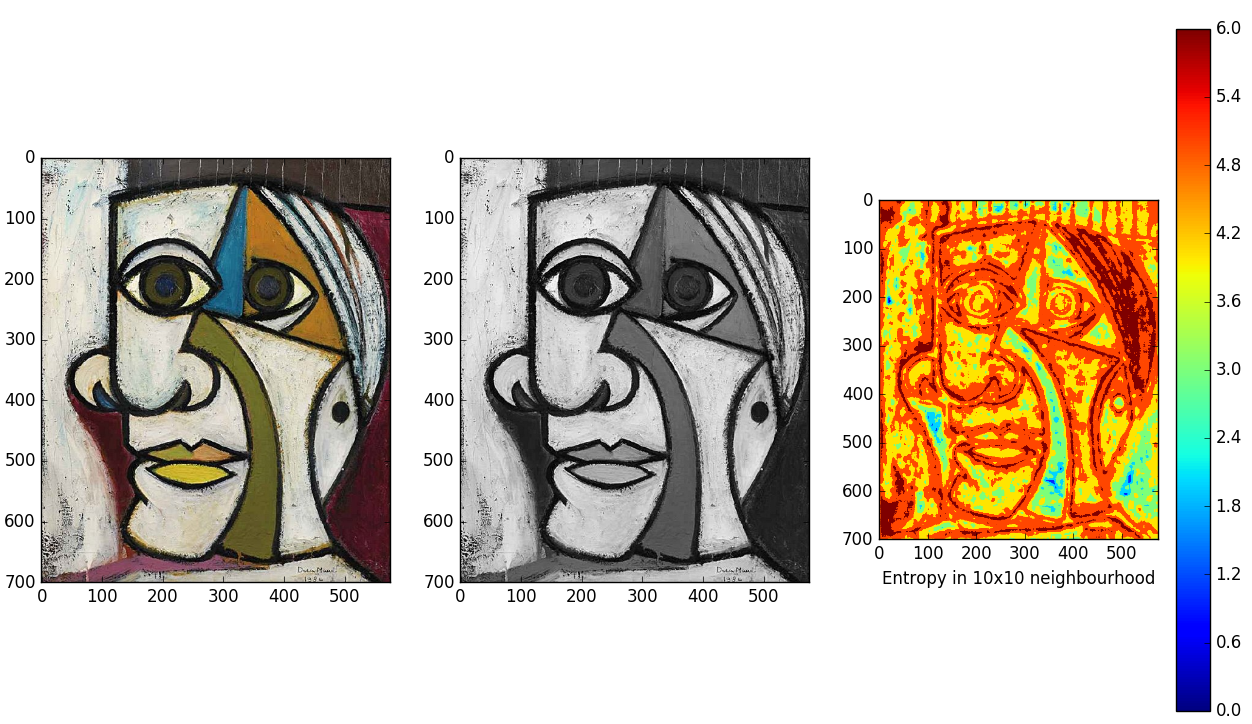
\includegraphics[scale = 0.35]{img/entropy_picasso}
\caption{Entropy of the Picasso, figure \ref{picasso}}
\label{entropy_picasso}
\end{figure} 

\begin{figure}[H]
\centering
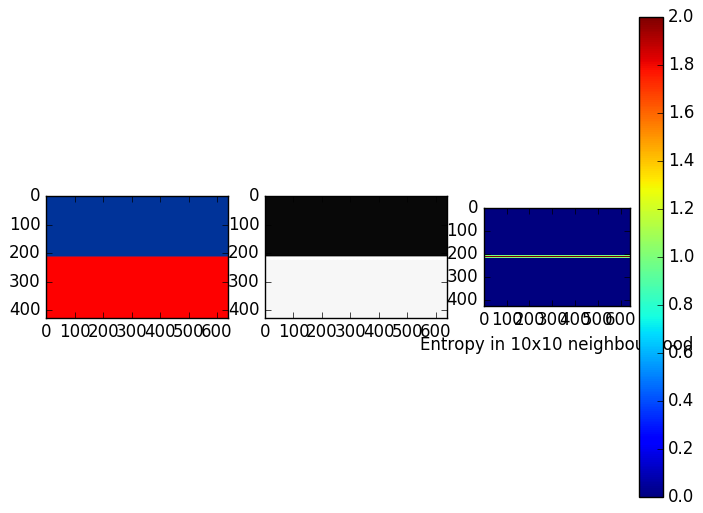
\includegraphics[scale = 0.54]{img/entropy_blue_red}
\caption{Entropy of a blue and red image}
\label{entropy_blue_red}
\end{figure} 
\newpage

\section{Text Processing Algorithms}

The field of text processing algorithms can be summarized as follows: a transformation where an image of some text is recognized and its meaning can be extracted. This concept is called Optical Character Recognition (OCR) [15].

\subsection{Pre-processing}

To increase the effectiveness of the OCR algorithms we can pre-process the images.
Several techniques can be used.

\paragraph{Layout analysis}

Often called 'zoning', this technique identifies columns, paragraphs, sections, etc as distinct blocks.

\paragraph{Character isolation}

If you want to apply OCR to every character seperatly (per-character OCR), this technique breaks multiple characters into single letters or characters.

\paragraph{Binarisation}

Converts the image from color to grayscale. It is a simple way to seperate the text from the background of the image. Most OCR algorithms work only on grayscale images since these images are easier to work with. 

\subsection{Character Recognition}

\subsubsection{Pattern Recognition}

One of the first techniques developed is pattern recognition, sometimes called matrix matching. This technique involves comparing an image of text to a previously stored glyph\footnote{An elemental symbol within an agreed set of symbols (alphabet), intended to represent a readable character.} on a pixel-by-pixel basis. This only works if the glyph and the input text are in the same font, same scale and if the input text can be isolated from the rest of the image.
\newline

This is very similar to supervised learning in classification. We have some learning data (the stored glyph) and we use this to get the correct results from unkown data.

\subsubsection{Feature Extraction}

This techinque uses 'features' as glyphs, for example, lines, closed loops, line intersection. Using these features instead of the complete glyph reduces dimensionality and makes the recognition computationally more efficient.
\newline

An example of an algorithm used is the k-nearest neighbour classification algorithm or $k$-NN. It is used to compare image features with stored glyph features and choose the nearset match. Traning data is needed, since it is a supervised learning algorithm. Important to notice is that the feature vectors are in a multidimensional feature space, each with a class label. Storing the vectors in a multidimensional space allows us to calculate the distances between vectors. This distance will be used to choose the best classification. A test sample (in this case a character to recognise) is classified by assigning the label of the feature vector which is most frequent among the $k$ training samples nearest to the test sample [16]. 
\newline

The Euclidian distance is commonly used to determine the distance between two continous samples. If the variables are discrete, which is the case in text classification, the overlap metric or Hamming distance is used. This metric is the number of positions at which the symbols to compare are different. In figure \ref{hamming} you can see an example of this metric. The distance between $100$ and $011$ is $3$, which is the number of sides of the cube you have to follow to get from $100$ to $001$ [17].
\newline

In figure \ref{kNN} you can see an example of the $k$-NN algorithm. The green circle is the test sample. To determine if it should be classified as a blue square or as a red triangle, we look at the number of occurences of the possible classifications in the circle. The solid line circle is the space created by the algorithm with $k = 3$. Now the green circle is seen as a red triangle, because there are two red triangles and only one blue square. If $k = 5$, the space created by k-NN is the dashed line circle. Now the algorithm would classify the green circle as a blue square because there are two red triangles and three blue squares in the circle. 

\begin{figure}[H]
\centering
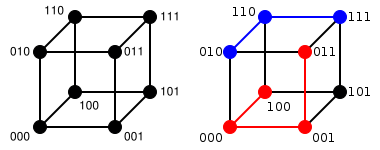
\includegraphics[scale = 0.7]{img/hamming}
\caption{Example of the Hamming metric}
\label{hamming}
\end{figure} 

\begin{figure}[H]
\centering
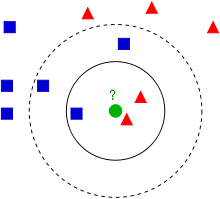
\includegraphics[scale = 0.6]{img/kNN}
\caption{Example of the $k$-NN algorithm}
\label{kNN}
\end{figure} 
	
\newpage

\begin{thebibliography}{1}

\bibitem{OpenImageR} Lampros Mouselimis {\em OpenPackageR, An Image Processing Toolkit} 2017

\bibitem{Convolution} R. Fisher, S. Perkins, A. Walker, E. Wolfart {\em Hypermedia Image Processing Reference} 2003

\bibitem{Frei_Chen_Sobel} Daniel R\'akos' blog (\url{http://rastergrid.com/blog/2011/01/frei-chen-edge-detector/}) 2011

\bibitem{Gaussian} University of Auckland, New Zealand, Computer Science course Computer Graphics and Image Processing {\em Gaussian Filtering} 2010

\bibitem{edge} Computaç\~ao Visual e Multimédia, course on Image Processing

\bibitem{prewitt} RoboRealm blog (\url{http://www.roborealm.com/help/Prewitt.php}) 2017

\bibitem{scharr} Jogn Costella's blog ( \url{http://johncostella.com/edgedetect/}) 2012

\bibitem{image filter} Simon Colton, Pedro Torres {\em Evolving Approximate Image Filters} 2009, Computational Creativity Group
Department of Computing, Imperial College London

\bibitem{hash} Dr. Neal Krawetz' blog (\url{http://www.hackerfactor.com/blog/?/archives/529-Kind-of-Like-That.html}) 2013

\bibitem{entropy} John Loomis' site (\url{http://www.johnloomis.org/ece563/notes/basics/entropy/entropy.html}) 1998

\bibitem{entropy} Kevin Meurer's blog (\url{http://kevinmeurer.com/a-simple-guide-to-entropy-based-discretization/}) 2015

\bibitem{entropy_python} Python Multimedia Codec Exercices Documentation (\url{https://www.hdm-stuttgart.de/~maucher/Python/MMCodecs/html/basicFunctions.html}) 2013

\bibitem{color} Ryan Walker's blogpost (\url{https://www.r-bloggers.com/color-quantization-in-r/}) 2016

\bibitem{noise} C. Solomon, T. Breckon {\em Fundamentals of Digital Image Processing: A Practical Approach with Examples in Matlab} 2011

\bibitem{OCR} \url{https://en.wikipedia.org/wiki/Optical_character_recognition}

\bibitem{kNN} \url{https://en.wikipedia.org/wiki/K-nearest_neighbors_algorithm}

\bibitem{hamming} \url{https://en.wikipedia.org/wiki/Hamming_distance}
\end{thebibliography}

\end{document}
